\documentclass[12pt]{article}
\usepackage[utf8]{inputenc}
\usepackage[english]{babel}
\usepackage{listings}
\usepackage{tikz}
\usepackage{amsmath,amssymb}

\usepackage{subcaption}

\tikzset{main node/.style={circle,fill=white!20,draw,minimum size=1cm,inner sep=0pt},}
\usepackage{verbatim}
\newcommand{\HRule}{\rule{\linewidth}{0.5mm}}

\begin{document}

\begin{center}
\textsc{\LARGE Principles of Computer System Design}\\[0.3cm] % Context
\HRule \\[0.4cm]
{ \huge \bfseries Assignment 3} % Main title
\HRule \\[0.4cm]
\large
Johannes de Fine Licht % Names
\\Philip Graae
\\Ola Rønning
\\\today
\end{center}
\section*{Recovery Concepts}
\subsection*{1.}
If a system implements force and no-stealing, the system will not have to implement \texttt{REDO} nor \texttt{UNDO}. The system will not have to implement \texttt{REDO} as the state of system is always consistent on the non-volatile memory, this is because writes are forced to write to the the non-volatile memory. As the system does not implement stealing; non-volatile storage will never have dirty cells, and hence there will be nothing to \texttt{UNDO} after a crash.
\subsection*{2.}
The difference between non-volatile and stable storage, is that stable storage can recover from media failure by implementing redundancy. Both kind of storage can recover from crashes. The final kind of storage, volatile storage, cannot recover from neither media failure nor crashes.
\subsection*{3.}
The two situations that will require the log tail to be forced to stable storage, are before a data page is written to non-volatile storage and when a transaction commits. The log tail must be forced to stable storage before a data page is written to ensure recoverability in case of a subsequent crash where the data page is lost. The log tail must furthermore be forced to stable storage when a transaction is committed to ensure the changes of a committed transaction can survive crashes. As volatile storage will not be recoverable from a crash, a record of the state of the system that the non-volatile storage represents after a crash is necessary. Hence to ensure the durability of the system, it is sufficient to maintain a record of state represented by the storage that will survive a crash, i.e. non-volatile storage.
\section*{ARIES}
\begin{table}[h!]
\begin{tabular*}{\textwidth}{@{\extracolsep{\fill}}lllll} 
\texttt{LOG}&&&& \\ 
&&&&\\ 
\texttt{LSN} & \texttt{LAST\_LSN} & \texttt{TRAN\_ID} & \texttt{TYPE} & \texttt{PAGE\_ID} \\
\texttt{1} & \texttt{-} & \texttt{-} & \texttt{begin CKPT} & \texttt{-} \\ 
\texttt{2} & \texttt{-} & \texttt{-} & \texttt{end CKPT} & \texttt{-} \\ 
\texttt{3} & \texttt{NULL} & \texttt{T1} & \texttt{update} & \texttt{P2} \\ 
\texttt{4} & \texttt{3} &\texttt{T1} & \texttt{update} & \texttt{P1} \\ 
\texttt{5} & \texttt{NULL} & \texttt{T2} & \texttt{update} & \texttt{P5} \\ 
\texttt{6} & \texttt{NULL} & \texttt{T3} & \texttt{update} & \texttt{P3} \\ 
\texttt{7} & \texttt{6} & \texttt{T3} & \texttt{commit} & \texttt{-} \\ 
\texttt{8} & \texttt{5} & \texttt{T2} & \texttt{update} & \texttt{P5} \\
\texttt{9} & \texttt{8} & \texttt{T2} & \texttt{update} & \texttt{P3} \\
\texttt{10} & \texttt{6} & \texttt{T3} & \texttt{END} & \texttt{-} \\ 
\end{tabular*}
\caption{The log records before a crash.}
\label{log}
\end{table} 
\subsection*{1.}
\begin{table}[h!]
\begin{tabular*}{\textwidth}{@{\extracolsep{\fill}}lllll} 
\texttt{Transaction table}&&&& \\ 
&&&&\\ 
\texttt{TRAN\_ID} & \texttt{Status} & \texttt{last\_LSN} \\
\texttt{T1} & \texttt{progress} & \texttt{4} \\ 
\texttt{T2} & \texttt{progress} & \texttt{9} \\ 
\end{tabular*}
\caption{The transaction table after the crash, based on the log, see table~\ref{log}.}
\label{trans}
\end{table}
\begin{table}
\begin{tabular*}{\textwidth}{@{\extracolsep{\fill}}lllll} 
\texttt{Dirty page table}&&&& \\ 
&&&&\\ 
\texttt{Page\_ID} & \texttt{recLSN} \\
\texttt{P1} & \texttt{4}\\ 
\texttt{P2} & \texttt{3}\\ 
\texttt{P3} & \texttt{6}\\ 
\texttt{P5} & \texttt{5}\\
\end{tabular*}
\caption{The dirty page table after the crash, based on the log, see table~\ref{log}.}
\label{dirty}
\end{table}
The transaction table, see table~\ref{trans}, is based on the log, see table~\ref{log}. Transaction three has ended and hence is not on the Transaction table, whilst transaction one and two are still in progress, when the crash occurs.\\
The dirty page table, see table~\ref{dirty}, is based on the log, see table~\ref{log}. The \texttt{recLSN} field represents the first log sequence number identifying a update dirtying a particular page. Pages one, two three and five was written to after the last checkpoint where the dirty page table was flushed.
\subsection*{2.}
The set of winner transaction are transactions that have committed and ended before the crash occurs, whilst the loser set represents the transactions that are still in progress. Hence the winner set for the log, see table~\ref{log}, is \{\texttt{T3}\} and the losers set is \{\texttt{T1}, \texttt{T2}\}.
\subsection*{3.}
The redo phase will begin at LSN three as this is the lowest LSN recorded in the dirty page table. The undo phase will ended at LSN three, the highest LSN will be picked and after the modification it identifies is undone its \texttt{LAST\_LSN} will be added until all transaction recorded in the Transaction table have \texttt{NULL} recorded in their \texttt{LAST\_LSN} field.
\subsection*{4.}
The set of LSNs that identify log records may need to be rewritten are \{3, 4, 8, 9\}. Log record three may need to be rewritten as it is on the dirty page table, see table~\ref{dirty}, its LSN is equal to the recorded recLSN on the dirty table. Lastly we are using ARIES and transaction one has not been committed. Log records three, four, eight and nine are in the set by a similar argument. 
\subsection*{5.}
The set of LSNs that identify log records that must be undone during the undo phase is \{9, 8, 5,4,3\}. These are the modification done by the loser transactions before the last checkpoint.
\subsection*{6.}
\begin{table}[h!]
\begin{tabular*}{\textwidth}{@{\extracolsep{\fill}}lllll} 
\texttt{LOG}&&&& \\ 
&&&&\\ 
\texttt{LSN} & \texttt{LAST\_LSN} & \texttt{TRAN\_ID} & \texttt{TYPE} & \texttt{PAGE\_ID} \\
\texttt{1} & \texttt{-} & \texttt{-} & \texttt{begin CKPT} & \texttt{-} \\ 
\texttt{2} & \texttt{-} & \texttt{-} & \texttt{end CKPT} & \texttt{-} \\ 
\texttt{3} & \texttt{NULL} & \texttt{T1} & \texttt{update} & \texttt{P2} \\ 
\texttt{4} & \texttt{3} &\texttt{T1} & \texttt{update} & \texttt{P1} \\ 
\texttt{5} & \texttt{NULL} & \texttt{T2} & \texttt{update} & \texttt{P5} \\ 
\texttt{6} & \texttt{NULL} & \texttt{T3} & \texttt{update} & \texttt{P3} \\ 
\texttt{7} & \texttt{6} & \texttt{T3} & \texttt{commit} & \texttt{-} \\ 
\texttt{8} & \texttt{5} & \texttt{T2} & \texttt{update} & \texttt{P5} \\
\texttt{9} & \texttt{8} & \texttt{T2} & \texttt{update} & \texttt{P3} \\
\texttt{10} & \texttt{6} & \texttt{T3} & \texttt{END} & \texttt{-} \\ 
\multicolumn{5}{c}{\texttt{CRASH, RESTART}}\\
\texttt{11} & \texttt{-} & \texttt{T2} & \texttt{CLR;undo LSN 9} & \texttt{P3} \\ 
\texttt{12} & \texttt{-} & \texttt{T2} & \texttt{CLR;undo LSN 8} & \texttt{P5} \\ 
\texttt{13} & \texttt{-} & \texttt{T2} & \texttt{CLR;undo LSN 5} & \texttt{P5} \\ 
\texttt{14} & \texttt{13} &\texttt{T2} & \texttt{END} & \texttt{-} \\ 
\texttt{15} & \texttt{-} & \texttt{T1} & \texttt{CLR;undo LSN 4} & \texttt{P1} \\ 
\texttt{16} & \texttt{-} & \texttt{T1} & \texttt{CLR;undo LSN 3} & \texttt{P2} \\ 
\texttt{17} & \texttt{16} & \texttt{T1} & \texttt{END} & \texttt{-} \\ 
\end{tabular*}
\caption{The log records until restart.}
\label{crs}
\end{table} 
The table~\ref{crs} represents the log after recovery has been completed. Neither the analysis nor redo phase will write anything to the log. The redo phase could write end type record if there were any committed transactions that had not been ended, however, this is not the case. The undo phase will iterate over all loser transactions undoing the highest current LSN until the \texttt{LAST\_LSN} is \texttt{NULL} by which the transaction will be ended.
\section*{Programming Task}
\section*{Discussion on the Performance Measurements}
\subsection*{1.}
\subsection*{2.}

\begin{figure}[htbp]
\begin{subfigure}[t]{0.5\textwidth}
\centering
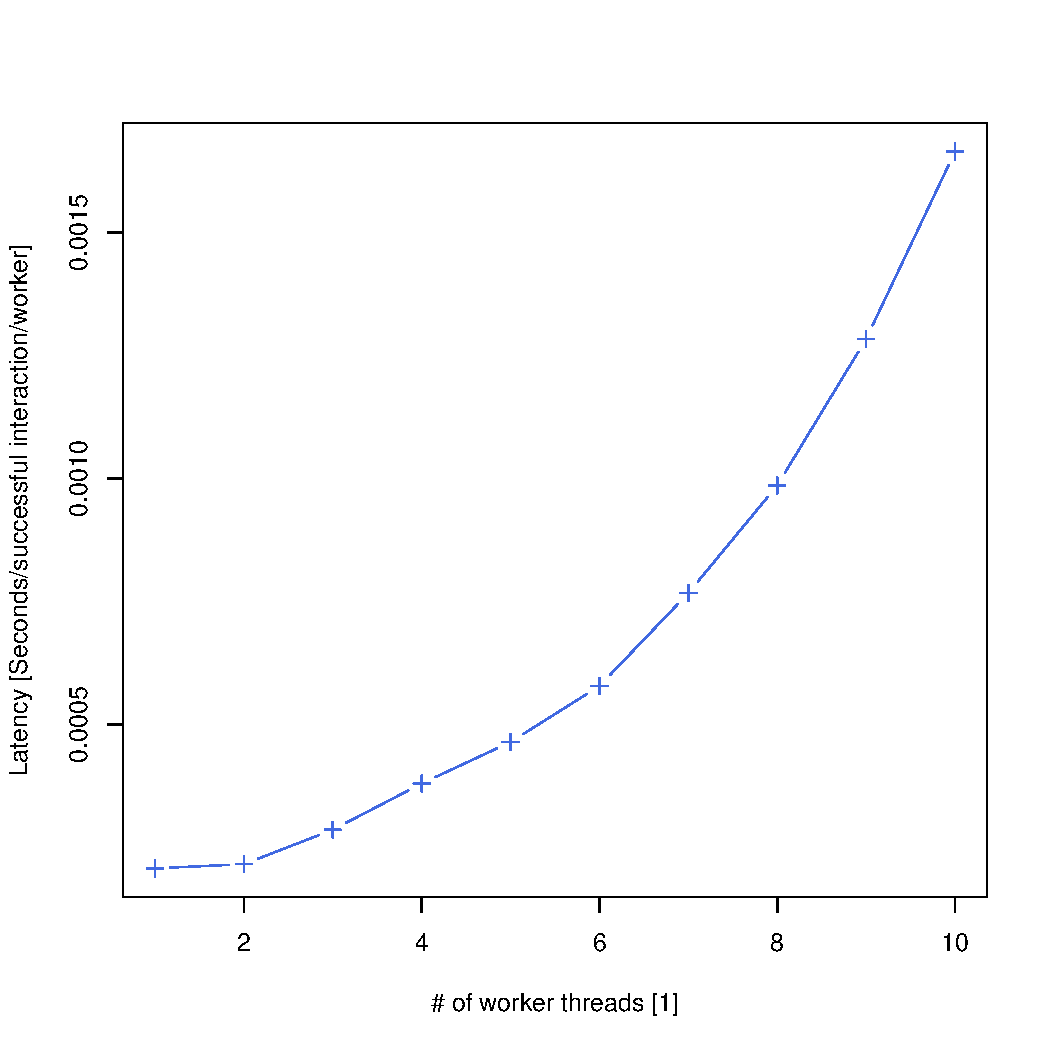
\includegraphics[scale=0.4]{latency.pdf}
\caption{Latency vs. number of worker threads}
\end{subfigure}
\begin{subfigure}[t]{0.5\textwidth}
\centering
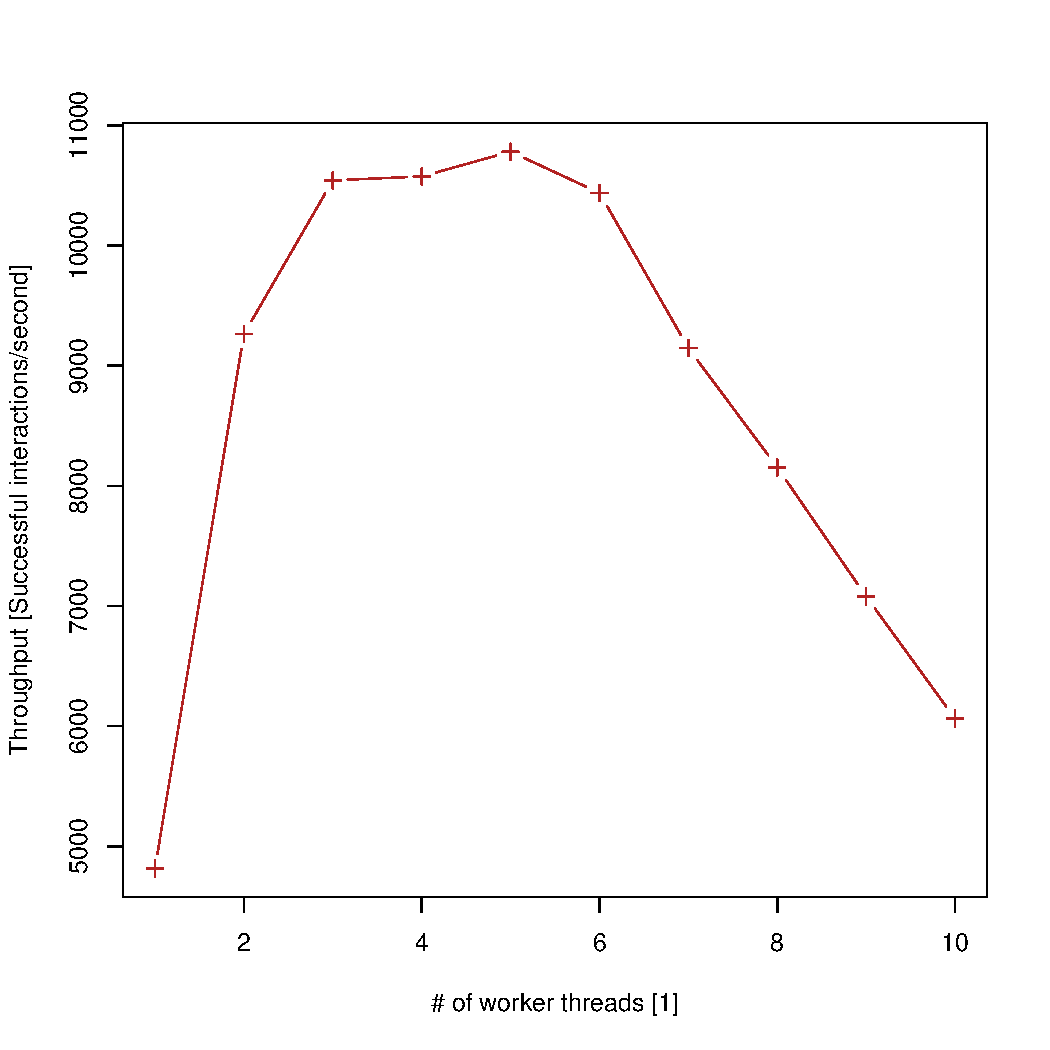
\includegraphics[scale=0.4]{throughput.pdf}
\caption{Throughput vs. number of worker threads.}
\end{subfigure}
\end{figure}

First looking at the local tests (red lines):
\\
\\
We see what looks like a polynomial increase in latency as a function of threads. We are not surprised to see an increase in latency when we add threads, since an individual thread will have to wait for more threads to be done with their transactions, before it can acquire a lock and do its own transaction. We suspect that the reason for polynomial increase, is that each thread on average will have to wait for half of all other threads minus itself to be done. For $n$ threads, this give us something like $n\cdot(n/2-1)$, which should give polynomial time.
\\
\\
We see that we have maximum throughput at 4-7 threads. The increase prior to this, could be explained by the rather naive assumption that more concurrency equals more performance, due to factors such as a better utilisation of available cores, hiding I/O and memory latency by scheduling other threads, and so forth. At higher numbers of threads however, we see a decline. Here, the negative scaling factors such as locking and thread management overhead, presumably become dominant over the positive scaling factors of increased concurrency mentioned before.
\\
\\


\subsection*{3.}
\end{document}
